\documentclass[12pt]{article}
\usepackage{lingmacros}
\usepackage{tree-dvips}
\usepackage{graphicx}
\usepackage{grffile}
\usepackage{cite}
\usepackage{float}

\begin{document}
\title{Notes for the continous control project}
\date{2018\\ November}
\author{Raphael Gross}
\maketitle




\section{Introduction}
This is the second project of the Udacity DRL course. My goal for this project is to get a better understanding of continuous control with deep reinforcement learning by implementing the  Deep Deterministic Policy Gradient (DDPG) algorithm in pytorch. In order to achieve my goal, I describe briefly the main features of the DDPG method, the Reacher environment used for testing the algorithm and finally, I show the results I obtained.


\section{State of the Art}

I used the DDPG algorithm to solve the Reacher environment. DDPG is a model-free, off-policy actor-critic algorithm that enables solving continuous action environment. 
DDPG is based on the deterministic policy gradient or DPG \cite{LHDWR14}.
DDPG has a parametrized actor function $\mu(s|{\theta}^{\mu})$ which specifies the current policy by deterministically mapping states to a specific action while the critic $Q(s,a)$ is learned using the Bellman equation.

DDPG uses some of the advantages of DQN such as sample replay and the target network.
Sample replay reduces correlations between sample. The replay buffer is constitued of tuples $(s,a,r,s')$  with $s$ the observations, $a$ actions, $r$ rewards and $s'$ the new states.
I stock the interaction between agents and the environment in the same replay buffer without distinction.

The DDPG model like DQN\cite{mnih2015humanlevel} uses a target network adapted to actor-critic and soft target updates for the network weights. We have an actor target $mu'$ and a critic target $Q'$. These two points increase the stability of the network and let it learn the action-value function. 

The principal issue in continuous action space is exploration. I define the exploration policy as the sum of the policy $\mu$ and some noise function $\mathcal{N}$ obtained using the Ornstein-Uhlenbeck process.


\section{Testing environment}
The environment I used to train and test my agent is called Reacher. In this environment, the agent control a double-jointed arm. The arm needs to reach a moving target location. For each step the agent manages to touch the target location, a reward of +0.1 is provided. Thus, the goal of my agent is to maintain as long and often as possible the arm hand on the target location.

The observation space is composed of 33 variables corresponding to the position, rotation, velocity, and angular velocities of the arm. Each action is determined by a vector of dimension 4 corresponding to the torque applied to the two joints. The action vector values are between -1.0 and 1.0.

For this project, I will use the multi-agent Unity environment. This environment is composed of 20 identical agents and each of them has its own copy of the environment. The task is episodic. After each episode, each agent gets a reward without discounting.  In order to solve the environment, the average score (all agents) needs to be greater than 30 over 100 consecutive episodes.

\begin{center}
\begin{figure}[H]
  \center
  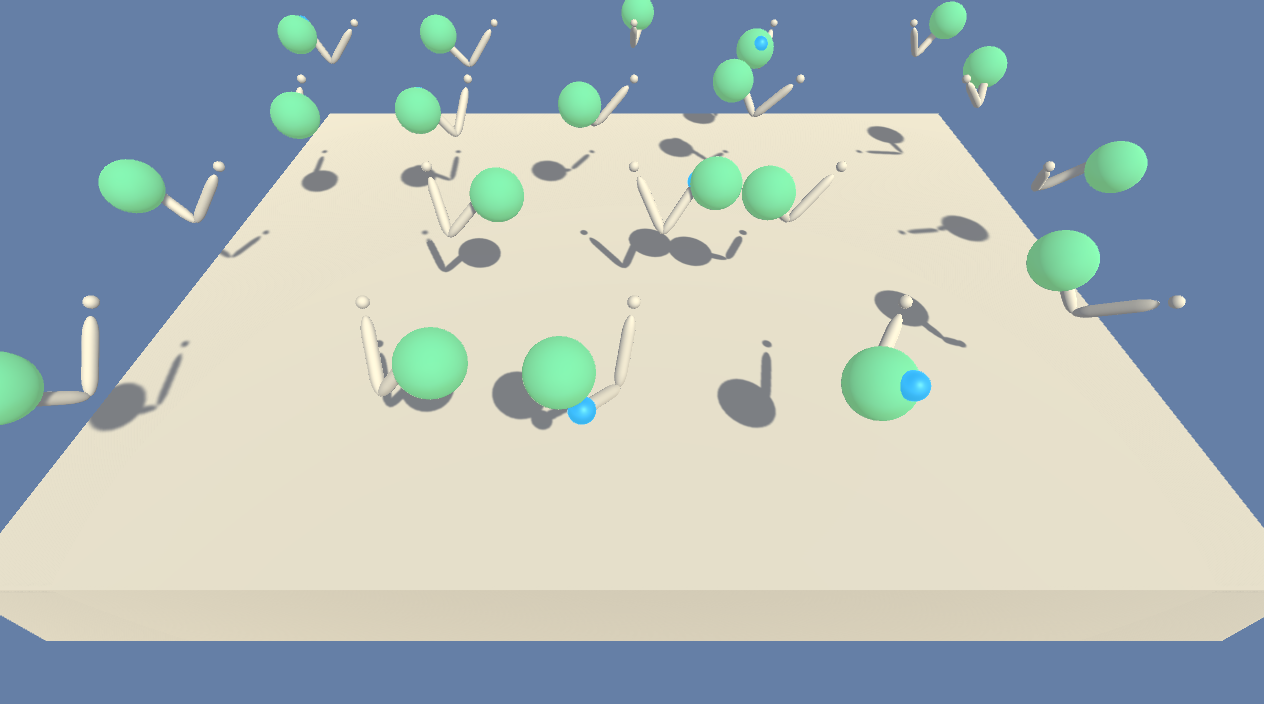
\includegraphics[width=0.7\textwidth]{../PNG/env.png}
  \caption{Reacher environment}
  \label{fig:reacher_environment}
\end{figure}
\end{center}


\section{Results} 
\subsection{Models}
he DDPG method is composed of two networks one for the actor and one for the critic.

\subsubsection{Actor}
The actor-network is composed of linear layers:

\subsubsection{Actor}
The actor network is composed of linear layers:
\begin{itemize}
\item fc1 : $nn.Linear(state\_size, fc1\_units)$
\item fc2 : $nn.Linear(fc1\_units, fc2\_units)$
\item fc3 : $nn.Linear(fc2\_units, action\_size)$
\end{itemize}

The weight for the first two hidden layers is initialized using a Xavier initialization.
The number of input and output nodes for the hidden layers is defined by the next parameters:

\begin{itemize}
\item $state\_size=33$
\item $fc1\_units=256$
\item $fc2\_units=128$
\item $action\_size=4$
\end{itemize}

In the forward pass, $fc1$ and $fc2$ are combined with a $ReLU$ rectifier. Finally, the policy is given after injecting $fc3$ into a tanh logistic sigmoid function.

\subsubsection{Critic}
The critic-network is composed of linear layers:

\begin{itemize}
\item $fc1 = nn.Linear(state\_size, fc1_units)$
\item $fc2 = nn.Linear(fc1\_units+action_size, fc2_units)$
\item $fc3 = nn.Linear(fc2\_units, 1)$
\end{itemize}
The number of input and output nodes for the hidden layers is defined by the next parameters:

\begin{itemize}
\item $state\_size=33$
\item $fc1\_units=256$
\item $fc2\_units=128$
\item $action\_size=4$
\end{itemize}

The weights for the first two hidden layers are initialized using a Xavier initialization.
The architecture of the critic is a bit unusual. The critic is used to estimate $Q(s, a(\mu))$. But, the action contribution is added to the network only after the first hidden layer.

The authors of the DDPG method\cite{LHDWR14} decided to concatenate the output of the first layer with the action just before the second hidden layer. One possible reason for this choice is to reduce the impact of the critic gradient on the actor computation during the backpropagation.


\begin{itemize}
\item $x\_s   = F.relu(self.fc1(state))$
\item $x\_s\_a = torch.cat((x\_s, action), dim=1)$
\item $x\_s\_a = F.relu(self.fc2(x\_s\_a))$
\item $Q\_s\_a  = self.fc3(x\_s\_a)$
\end{itemize}

\subsection{Parameters}
The best result I obtained for the DDPG method was with the next parameters values:

\begin{itemize}
\item MEMORY SIZE = int(1e5) (replay buffer size)
\item BATCH SIZE = 128  (minibatch size)
\item GAMMA = 0.99  (discount factor)
\item TAU = 1e-3  (parameter value used for the soft update of the target weights)
\item LR\_ACTOR = 8e-5  (learning rate for actor)
\item LR\_CRITIC = 8e-5  (learning rate for critic)
\item UPDATE EVERY = 1  (how often the target network is updated)
\end{itemize}


\subsection{Score}
In Figure ~\ref{fig:average_score_all}, I plot the score fo obtained by each agent at each episode. The score corresponds to the sum of all the reward an agent obtained during an episode. The algorithm took 135 episodes to converge. 

\begin{center}
\begin{figure}[H]
  \center
  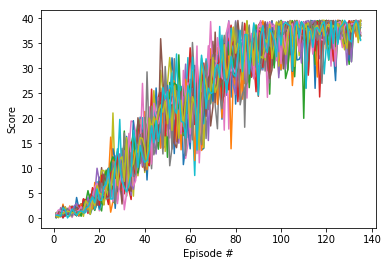
\includegraphics[width=0.7\textwidth]{../PNG/average_score_all.png}
  \caption{Score for each agent}
  \label{fig:average_score_all}
\end{figure}
\end{center}

In Figure ~\ref{fig:average_score}, I display the mean score at each episode.
\subsection{Score}
\begin{center}
\begin{figure}[H]
  \center
  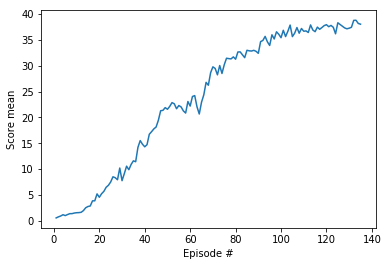
\includegraphics[width=0.7\textwidth]{../PNG/average_score.png}
  \caption{Average score}
  \label{fig:average_score}
\end{figure}
\end{center}

\subsection{Future improvement}
For now, I only covered the DDPG\cite{LillicrapHPHETS15} algorithm. But, my ambition is to finish the PPO method\cite{ClaveraRS0AA18} I started to implement for continuous action and also look into A3C\cite{MnihBMGLHSK16}, A2C\cite{MnihBMGLHSK16} and D4PG\cite{Barth2018}. i will also try to solve other environment such as the Crawler environment.
\bibliography{bib}
\bibliographystyle{plain}

\end{document}


